% ****** Start of file apssamp.tex ******
%
%   This file is part of the APS files in the REVTeX 4.2 distribution.
%   Version 4.2a of REVTeX, December 2014
%
%   Copyright (c) 2014 The American Physical Society.
%
%   See the REVTeX 4 README file for restrictions and more information.
%
% TeX'ing this file requires that you have AMS-LaTeX 2.0 installed
% as well as the rest of the prerequisites for REVTeX 4.2
%
% See the REVTeX 4 README file
% It also requires running BibTeX. The commands are as follows:
%
%  1)  latex apssamp.tex
%  2)  bibtex apssamp
%  3)  latex apssamp.tex
%  4)  latex apssamp.tex
%
\documentclass[%
 reprint,
%superscriptaddress,
%groupedaddress,
%unsortedaddress,
%runinaddress,
%frontmatterverbose,
%preprint,
%preprintnumbers,
%nofootinbib,
%nobibnotes,
%bibnotes,
 amsmath,amssymb,
 aps,
%pra,
%prb,
%rmp,
%prstab,
%prstper,
%floatfix,
]{revtex4-2}

\usepackage{graphicx}% Include figure files
\usepackage{dcolumn}% Align table columns on decimal point
\usepackage{bm}% bold math
%\usepackage{hyperref}% add hypertext capabilities
%\usepackage[mathlines]{lineno}% Enable numbering of text and display math
%\linenumbers\relax % Commence numbering lines

%\usepackage[showframe,%Uncomment any one of the following lines to test
%%scale=0.7, marginratio={1:1, 2:3}, ignoreall,% default settings
%%text={7in,10in},centering,
%%margin=1.5in,
%%total={6.5in,8.75in}, top=1.2in, left=0.9in, includefoot,
%%height=10in,a5paper,hmargin={3cm,0.8in},
%]{geometry}

\begin{document}

\preprint{APS/123-QED}

\title{Summary of 'Update of the $B^0 \longrightarrow K*^0\mu^+\mu^-$ angular analysis at LHCb'\\with Forced Linebreak}% Force line breaks with \\
\thanks{A footnote to the article title}%

\author{Ann Author}
 \altaffiliation[Also at ]{Physics Department, XYZ University.}%Lines break automatically or can be forced with \\
\author{Second Author}%
 \email{Second.Author@institution.edu}
\affiliation{%
 Authors' institution and/or address\\
 This line break forced with \textbackslash\textbackslash
}%

\collaboration{LHCb Collaboration}%\noaffiliation

\author{Charlie Author}
 \homepage{http://www.Second.institution.edu/~Charlie.Author}
\affiliation{
 Second institution and/or address\\
 This line break forced% with \\
}%
\affiliation{
 Third institution, the second for Charlie Author
}%
\author{Delta Author}
\affiliation{%
 Authors' institution and/or address\\
 This line break forced with \textbackslash\textbackslash
}%

\collaboration{CLEO Collaboration}%\noaffiliation

\date{\today}% It is always \today, today,
             %  but any date may be explicitly specified

\begin{abstract}
An article usually includes an abstract, a concise summary of the work
covered at length in the main body of the article.
\begin{description}
\item[Usage]
Secondary publications and information retrieval purposes.
\item[Structure]
You may use the \texttt{description} environment to structure your abstract;
use the optional argument of the \verb+\item+ command to give the category of each item.
\end{description}
\end{abstract}


\maketitle

In the search for new physics, processes that are supressed in the standard model and therefor especially sensitive to physics beyond the
standard model are closely examined. The $b \longrightarrow s\mu^+\mu^-$ transition is a flavor changing neutral current (FCNC) and only occurs on
loop level in feynman diagramms, which makes it susceptible for finding new processes not described in the standard model. Such a
transition occurs in the decay of a $B^0$-meson into $K^{*0}\mu^+\mu^-$ and can be described with effective field theories on a given energy scale.
Loops in the penguin diagramm can be replaced with effective couplings corresponding to the Wilson coefficients $C_i$. As they are sensitive to
new physics comparing theoretical expectations with measurements is of high interest. An effective Hamiltonian containing the
combination of the Wilson coefficients and low energy QCD operators $O_i$ with large theory uncertainties.

The angular analysis is the measurement of the decay rate of a process as a function of the angles of the final decay products. As these
measurements can give access to a large range of observables with a reduced theory uncertainty, it can help
to deduce the nature of new physics models.

Since the FCNC from a b-Quark to an s-Quark lead to the production of an $K^{*0}$ meson in the process, analysing its angular structure is
vital. The $K^{*0}$ meson is a vector with spin 1 and can be easily reconstructed at LHCb via $K^{*0} \longrightarrow K^+\pi^-$.

Tension within the standard model arises with the measurement of the $C_9$ coefficient, which is involved in loop proceses.
Its measured value deviates $3.4\sigma$ from the standard model in the last LHCb result from 2016
under the assumption that the observation can be explained solely with the shift of $Re(C_9)$.

Global fits performed by various different experiments in 2019 show 3-5$\sigma$ deviations in $Re(C_9)$ favouring a shift of the
Wilson coefficient. The new physics component of $C_{10}$ for muons, which is also involved in the loop process of the penguin diagramm, was
plotted against $C_19$ shown in figure \ref{fig:shift}.


\begin{figure}[b]
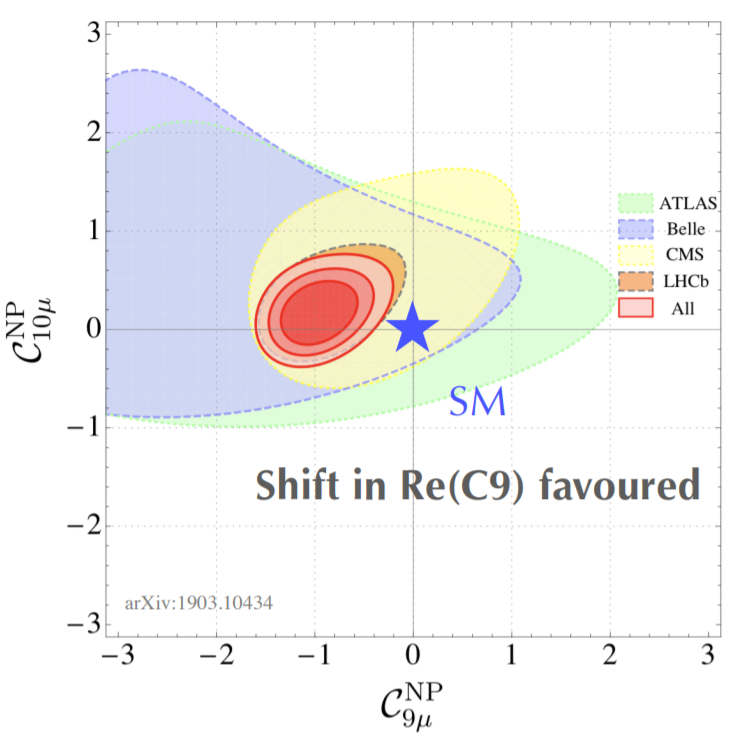
\includegraphics{shift}
\caption{\label{fig:shift}}
\end{figure}


Analysed data includes Run from LhCb in 2011 and 2012, as well as 2016 data. With an increased center of mass energy of 13 TeV in
comparison to 7 and 8 TeV of the earlier run, the added 2016 data nearly doubles the statistic reaching a
luminosity of 4.7 fb$^{-1}$.

The selection of candidates requires a small impact parameter for B mesons and a large one for the daughter products. These
requirements favours candidates coming directly from primary vertices. Particle identification is necessary to suppress peaking
backgrounds from anti B mesons and anti lambda baryons for example, as their decay products contain $\pi^-$ and $K^+$, which
leads to misidentification.

To detect the final state of the $b \longrightarrow s$ transition, the final state of $J/\psi$ has to be taken into account as
it is indistinguishable from the FCNC. Regions of interest in the $\text{d}\Gamma/q^2$ spectrum is therefor split
into three parts, which the two different charmonium states $J/\psi(1S)$ and $J/\psi(2s)$ can occupy.
The analysis is performed blind over an energy intervall of [0.1, 19] GeV$^2$ with mostly narrow and two wide bins with
the two charmonium regions from [8.0, 11.0] and [12.5, 15.0] GeV$^2$ serving as control channels.





\bibliography{apssamp}% Produces the bibliography via BibTeX.

\end{document}
%
% ****** End of file apssamp.tex ******
